\label{sec:particle_improves}
\begin{figure}[H]
\centering
\begin{subfigure}[b]{0.45\textwidth}
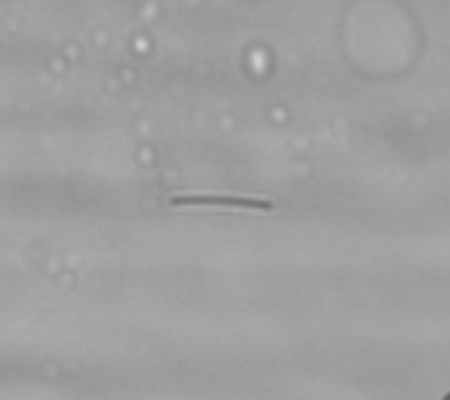
\includegraphics[width=0.9\textwidth]{figures/improvements/oldparticle2.png}
\caption{Particle 13 from July 2012}
\end{subfigure}
\begin{subfigure}[b]{0.45\textwidth}
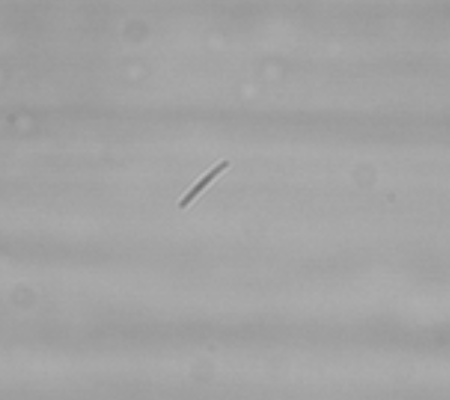
\includegraphics[width=0.9\textwidth]{figures/improvements/oldparticle3.png}
\caption{Particle 22 from July 2012}
\end{subfigure}
\caption{Two typical particles from the previous setup. Note that these particles are selected for being among the most symmetric in the sample and yet they are noticeably bent.}
\label{fig:oldparticles}
\end{figure}



In order to solve the issues with the polymer particles were replaced with glass particles from Nippon Glass, Japan \cite{Particles}. 

These new particles are made from LCD spacing rods that are broken into pieces. This means that they are essentially broken cylinders with very homogeneous widths but some variation in length. Two different batches of particles were used, one with a $3\mu m$ diameter and one batch with $5 \mu m$ diameter. All the measurements presented in this hesis are using the $3 \mu m$ width particles. This is primarily as they were more easily controlled with the optical tweezers and because they sink or float more slowly. 

The symmetries of the particles were investigated with help from Stefan Gustafsson by taking images with an 
ESEM (Environmental Scanning Electron Microscope) shown in Figure \ref{fig:particlepictures}. We see that the 
particles are uniformly smooth along the sides but have varyingly jagged edges causing different degrees of asymmetry. 

Figure \ref{fig:roundparticle} shows a particle along the main axis and we see that it is circular shape
with no discernible deformation or asymmetry whereas Figure \ref{fig:particlepictures} show the jagged edges of several particles. 


\begin{figure}[H]
\centering
\begin{subfigure}[3a]{0.40\textwidth}
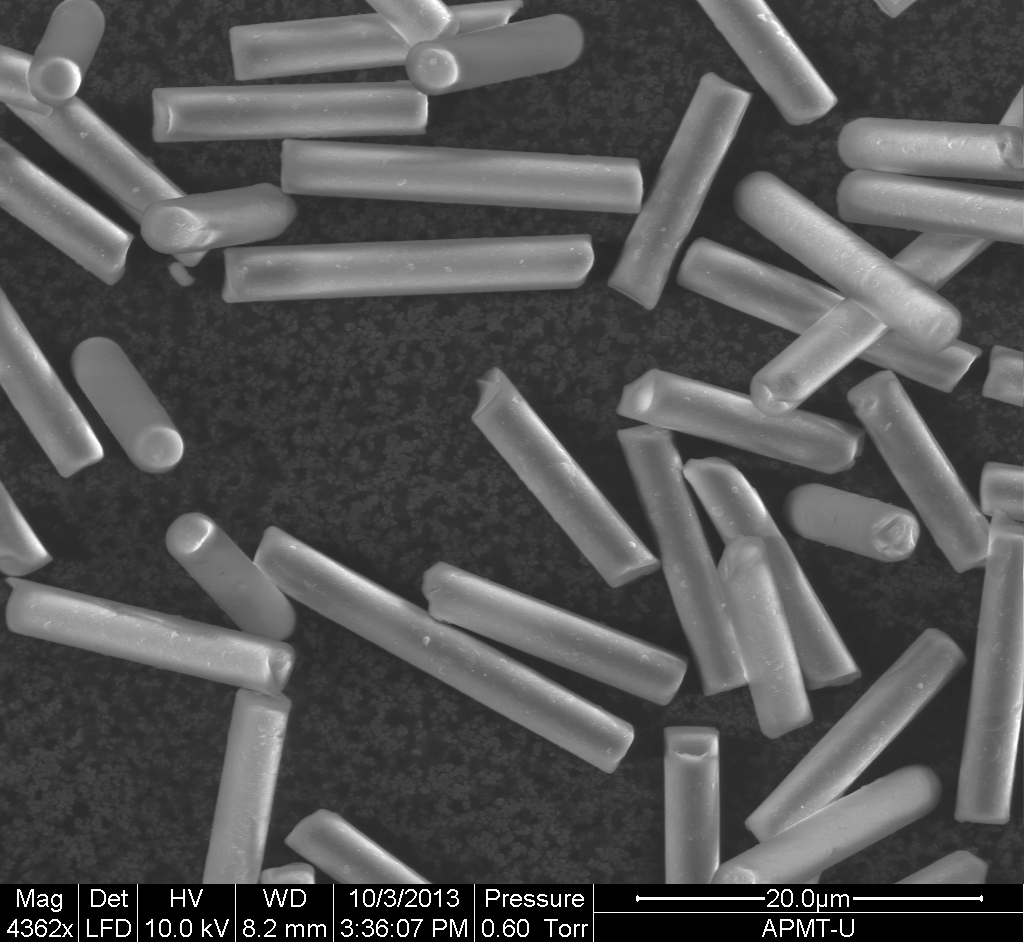
\includegraphics[width=\textwidth]{figures/method/semizoomed.png}
\caption{A detailed view \\ of a number of particles.}
\end{subfigure}\hspace{1em}%
\begin{subfigure}[3b]{0.40\textwidth}
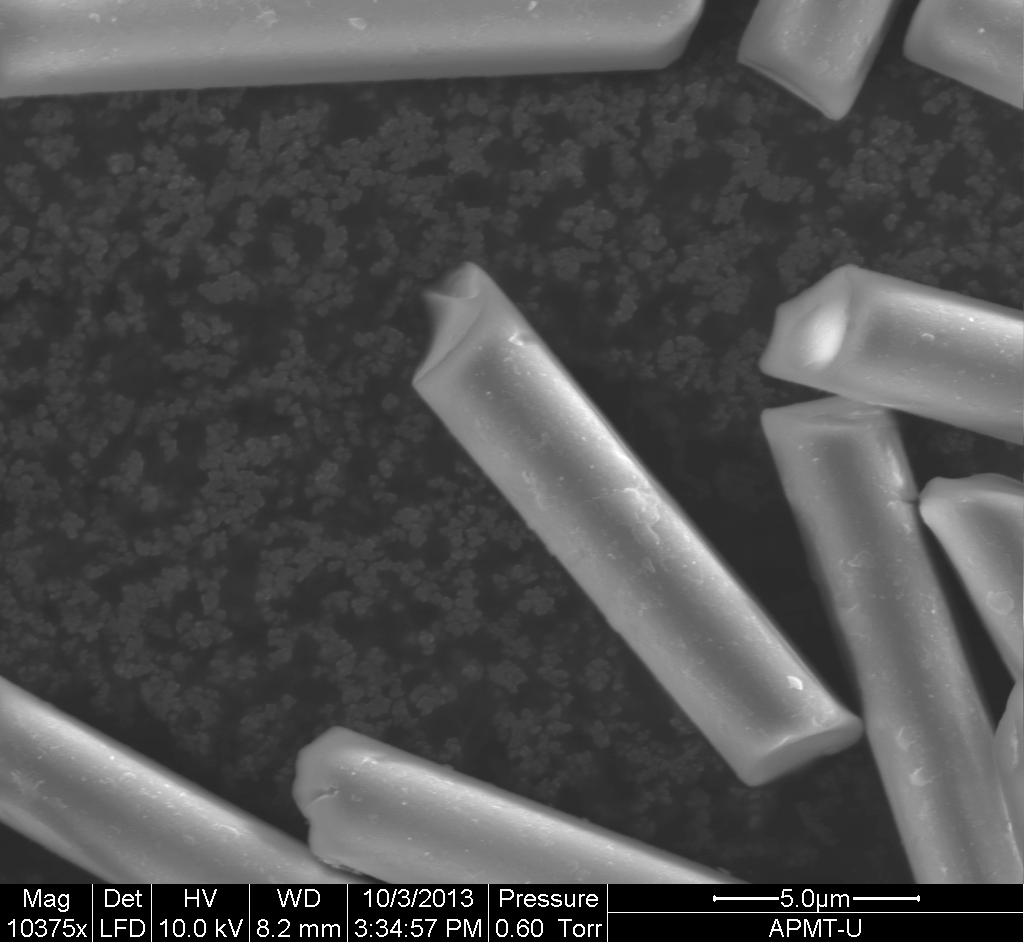
\includegraphics[width=\textwidth]{figures/method/zoomedbroken.png}
\caption{The jagged edge of a particle \\ in detail.}
\end{subfigure}
\caption{Pictures of the glass particles that were used. Their width is uniform and there is a noticeable variation in asymmetry. Some particles show very clearly jagged edges while other appear very smooth. This suggests that they should have quite different $\epsilon$ and then exhibit quite different behaviour. Obtained with the help of Stefan Gustafsson}
\label{fig:particlepictures}
\end{figure}
 
\begin{figure}[H]
\centering
\begin{subfigure}[3a]{0.40\textwidth}
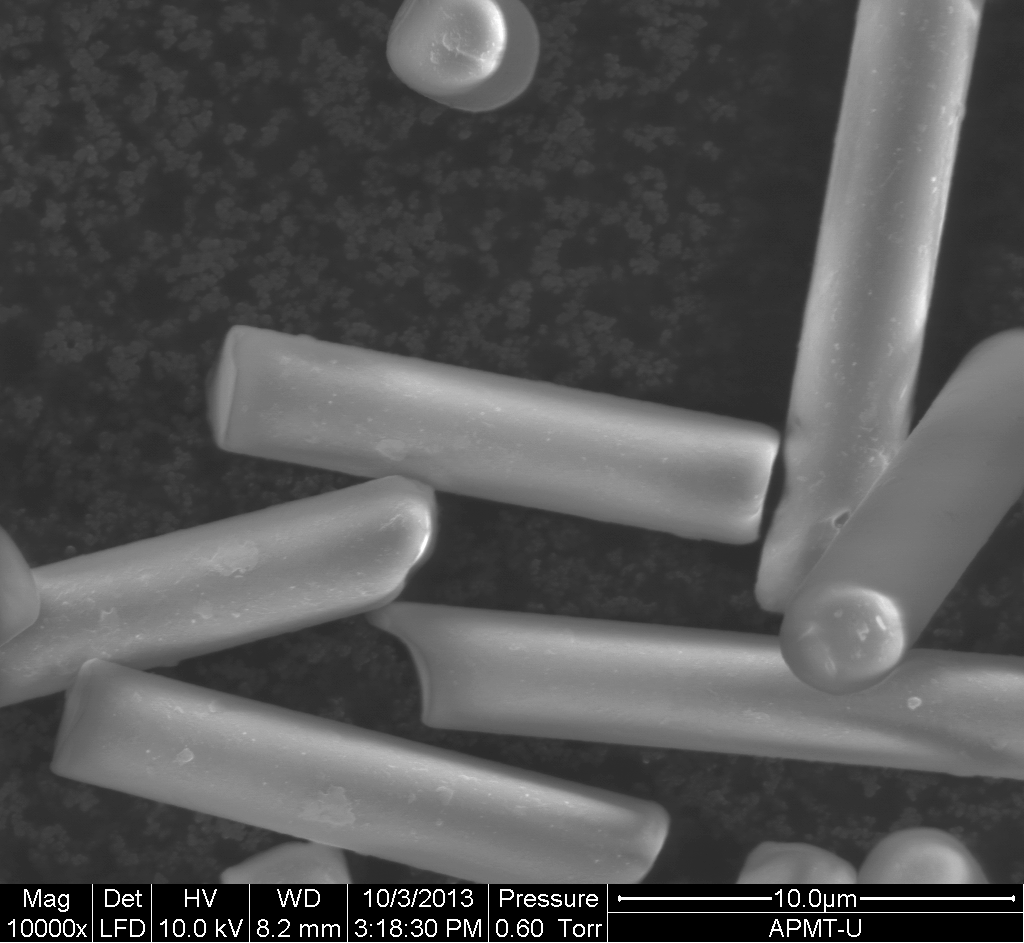
\includegraphics[width=\textwidth]{figures/method/symmetric.png}
\caption{What appears to be a highly \\ symmetric particle.}\label{fig:symmetricparticle}
\end{subfigure}\hspace{1em}%
\begin{subfigure}[3b]{0.40\textwidth}
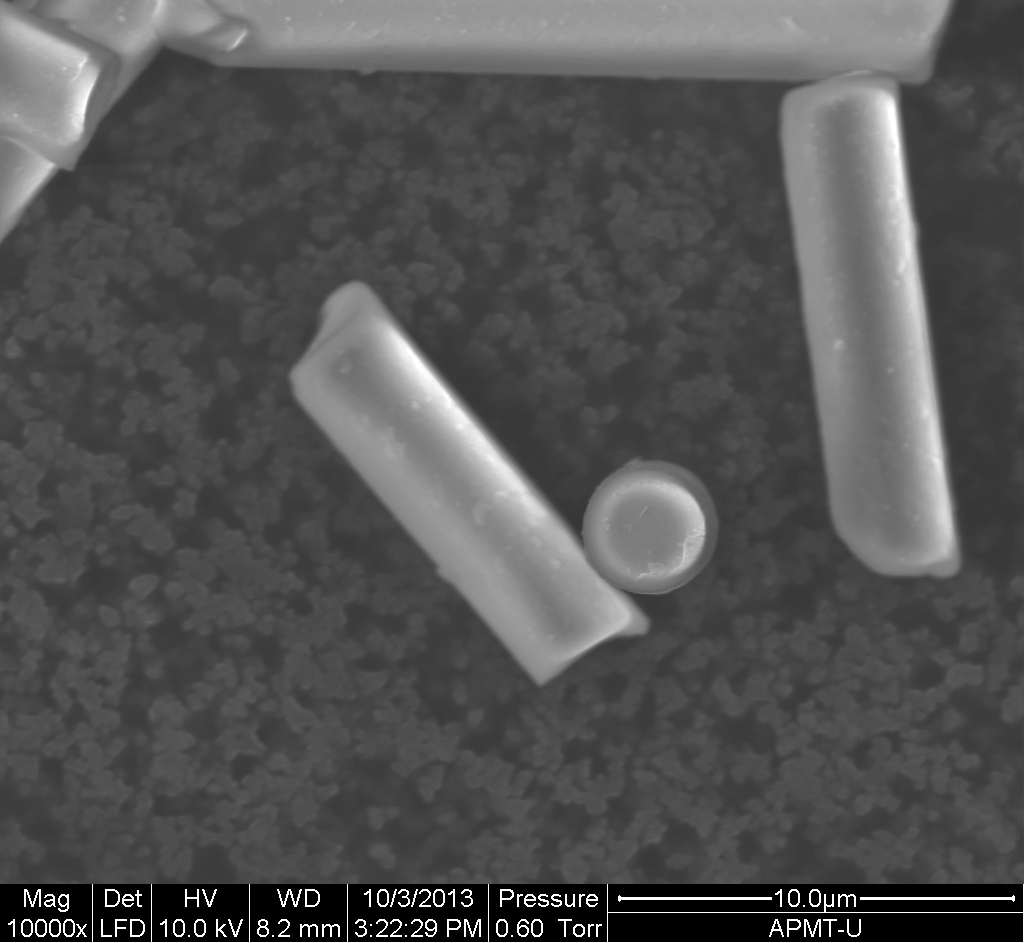
\includegraphics[width=\textwidth]{figures/method/round.png}
\caption{A top down view of a particle.}\label{fig:roundparticle}
\end{subfigure}
\caption{Pictures highlighting the roundness of the particles as well as the apparent symmetry of some particles. Obtained with the help of Stefan Gustafsson}
\label{fig:particlepictures2}
\end{figure}

Figure \ref{fig:roundparticle} and \ref{fig:symmetricparticle} are the same as can be seen in Laas~\cite{alexanderThesis} Figure 5.2(c) and 5.2(b) respectively. 

The particles satisfy the symmetry conditions but are made of glass with a density of approximately 
\unit[2.57]{g/cm$^3$} at \unit[20]{C$^\circ$}. This is significantly higher than that of water with a density of 
\unit[1]{g/cm$^3$} at \unit[20]{C$^\circ$} and glycerol with a density of \unit[1.5]{g/cm$^3$}. In order to keep the particles buoyant the water soluble Sodium metatungstate is added to the liquid. Sodium metatungstate dissolved in water has a density of \unit[2.94]{g/cm$^3$} at \unit[20]{C$^\circ$} when fully saturated. To increase the viscosity of the liquid around 8\% glycerol is added and the liquid was measured using a MCR 302 rheometer to have a dynamic viscosity of \unit[$24\cdot 10^{-3}$]{Pa s}.

The problem with using these cylindrical particles is that the asymmetric cylinders with jagged edges do not have the same symmetries as the triaxial particles. The triaxial particles with distinct $a_2$ and $a_3$ have $2$-fold rotational symmetry around every axis whereas this is not true for the cylinders. We do not know how this effects the equations of motion and in turn the orbits, Poincaré maps and the winding numbers. We assume that we can approximate a jagged cylinder with a triaxial particle and further theoretical development will prove if this is correct or not.
